%% ─────────────────────────────────────────────────────────────────────────────
%% main.tex — Full manuscript (Introduction, Methods, Results,
%%            Discussion, Conclusion)
%% Nature-style, numbered superscript citations in order of appearance
%% Compile: pdflatex main.tex  (figures/ must be in same directory)
%% ─────────────────────────────────────────────────────────────────────────────

\documentclass[12pt]{article}

%% ── Packages ─────────────────────────────────────────────────────────────────
\usepackage[T1]{fontenc}
\usepackage[utf8]{inputenc}
\usepackage{mathptmx}
\usepackage[scaled=0.90]{helvet}
\usepackage{microtype}
\usepackage{geometry}
\usepackage{graphicx}
\usepackage{booktabs}
\usepackage{tabularx}
\usepackage{multirow}
\usepackage{siunitx}
\usepackage{amsmath,amssymb}
\usepackage{caption}
\usepackage{subcaption}
\usepackage{float}
\usepackage{xcolor}
\usepackage[numbers,super,sort&compress]{natbib}   % Nature-style superscripts
\usepackage{hyperref}
\usepackage{parskip}
\usepackage{setspace}
\usepackage{enumitem}
\usepackage{placeins}

%% ── Page geometry ────────────────────────────────────────────────────────────
\geometry{
  paperwidth=210mm, paperheight=297mm,
  top=25mm, bottom=25mm, left=25mm, right=25mm,
}

%% ── Caption style ────────────────────────────────────────────────────────────
\captionsetup{
  font={small}, labelfont={bf,small}, format=plain,
  justification=justified, singlelinecheck=false, skip=4pt,
}

%% ── Hyperref ─────────────────────────────────────────────────────────────────
\hypersetup{
  colorlinks=true, linkcolor=black, citecolor=black, urlcolor=black,
}

%% ── siunitx ──────────────────────────────────────────────────────────────────
\sisetup{
  separate-uncertainty=true, uncertainty-mode=separate,
  table-align-uncertainty=true,
}

%% ── Section headings ─────────────────────────────────────────────────────────
\makeatletter
\renewcommand\section{\@startsection{section}{1}{\z@}%
  {-9pt plus -2pt minus -1pt}{3pt plus 1pt}%
  {\normalfont\large\bfseries}}
\renewcommand\subsection{\@startsection{subsection}{2}{\z@}%
  {-6pt plus -1pt minus -1pt}{2pt plus 1pt}%
  {\normalfont\normalsize\bfseries}}
\renewcommand\subsubsection{\@startsection{subsubsection}{3}{\z@}%
  {-4pt plus -1pt minus -1pt}{1pt}%
  {\normalfont\normalsize\itshape}}
\makeatother

%% ─────────────────────────────────────────────────────────────────────────────
\begin{document}
\singlespacing

%% ── Title block ──────────────────────────────────────────────────────────────
\begin{center}
  {\LARGE\bfseries
    When Does Posterior Belief Updating Improve Decisions?\\[6pt]
    Evidence from a Controlled Sequential Hidden-Information Testbed}\\[14pt]

  \renewcommand{\thefootnote}{\fnsymbol{footnote}}
  {\large Kevin Song\footnote{Corresponding author.
    Email: \href{mailto:kmsong@uab.edu}{kmsong@uab.edu}}
    \quad and \quad John Zhang}\\[6pt]
  \renewcommand{\thefootnote}{\arabic{footnote}}

  {\normalsize\itshape
    Department of Biomedical Engineering,
    The University of Alabama at Birmingham}\\[6pt]

  {\small March 18, 2026}\\[14pt]
\end{center}

\hrule height 0.8pt
\vspace{8pt}

\begin{center}
  \begin{minipage}{0.88\textwidth}
    \small\setstretch{1.15}
    \textbf{Abstract.}
    A foundational question in sequential decision-making is whether
    explicitly inferring an opponent's latent state -- through Bayesian
    posterior updating -- improves decisions beyond what is achievable
    with a well-calibrated static prior.
    We investigate this question in a controlled synthetic testbed:
    a heads-up turn-river no-limit Texas Hold'em subgame in which
    three agents compete across \num{75000} simulated hands.
    A fixed-rule Heuristic, a static-prior expected-value (Static-EV)
    agent, and a Bayesian-updating expected-value (Belief-EV) agent
    face off against seven parameterised opponent families, including
    two families held out from all development.
    Both EV agents dramatically outperform the Heuristic by
    $\approx$77 chips per hand ($\approx$79\%), establishing the
    primacy of principled expected-value reasoning over rule-based
    heuristics.
    Strikingly, however, the Static-EV agent outperforms the
    Belief-EV agent in direct head-to-head competition by
    9.9--13.1 chips per hand ($p \leq 0.034$, paired $t$-test),
    falsifying the central hypothesis.
    Analysis of per-decision posterior entropy reveals that Bayesian
    updates provide negligible discriminating signal
    ($H \approx 1.91$ bits, against a maximum of $1.95$ bits for
    seven equiprobable classes), leaving the posterior near-uniform
    and rendering updates a net liability.
    Neither EV agent loses performance on held-out opponent families,
    and dynamic belief tracking confers no robustness advantage.
    These findings identify the conditions under which hidden-state
    inference is harmful versus beneficial, and carry direct
    implications for the design of AI agents, fraud-detection
    systems, market-making algorithms, and clinical decision-support
    tools.
  \end{minipage}
\end{center}

\vspace{8pt}
\hrule height 0.4pt

%% ─────────────────────────────────────────────────────────────────────────────
%%  INTRODUCTION
%% ─────────────────────────────────────────────────────────────────────────────
\newpage
\doublespacing

\section{Introduction}

Sequential decision-making under hidden information is a central
challenge in artificial intelligence, game theory, and operations
research\cite{osborne1994course,pearl1988probabilistic}.
When an agent cannot directly observe an opponent's private state --
their intentions, resources, or information -- the rational response
is to maintain a probability distribution over that state and update
it as new evidence arrives\cite{pearl1988probabilistic,murphy2012ml}.
This Bayesian programme is theoretically well-motivated: an agent
with a perfectly accurate posterior over hidden states will, in
principle, make strictly better decisions than one operating from
a fixed prior\cite{koller1992complexity}.

In practice, however, belief updating carries costs.
The posterior is only as good as the \emph{response model}
$P(\text{action} \mid \text{hidden state})$ used to interpret
observed actions\cite{albrecht2018survey}.
When this model is misspecified -- when the opponent does not behave
as assumed -- Bayesian updates can push the posterior in the wrong
direction, compounding errors rather than resolving them\cite{gal2016dropout}.
The question of \emph{when} dynamic belief inference actually
improves decisions, and when it is merely costly overhead, remains
poorly understood in practice.

Poker has long served as a canonical testbed for sequential
decision-making under hidden information\cite{chen2006mathematics,
bowling2015holdem,brown2019superhuman}.
Its structure -- private hole cards, sequential betting, and
deterministic showdown resolution -- provides a clean formal
setting in which hidden-state inference is necessary, tractable,
and directly measurable\cite{koller1992complexity,zinkevich2007cfr}.
Recent superhuman systems such as Libratus and Pluribus
solve poker through counterfactual regret minimisation rather than
explicit belief tracking\cite{zinkevich2007cfr,brown2019superhuman},
raising the question of whether principled EV reasoning alone
suffices, even in settings with meaningful hidden information.

More broadly, the question maps onto a recurring debate in
multi-agent systems\cite{albrecht2018survey,tuyls2012multiagent}
and appears concretely in fraud detection (sequential account-state
inference\cite{dalpozzolo2015fraud}), financial market making
(belief updating over counterparty type\cite{glosten1985bid}),
clinical decision support (sequential Bayesian diagnosis\cite{obermeyer2016predicting}),
and autonomous vehicle intent
prediction\cite{bard2020hanabi,silver2016alphago}.
In each domain, a practitioner must decide whether to invest in
a dynamic opponent model or rely on a well-tuned static prior.

We address this question with a controlled experiment.
We build a turn-river Hold'em simulator and compare three
agents -- a rule-based Heuristic, a Static-EV agent with a fixed
uniform prior, and a Belief-EV agent that applies Bayes'
theorem\cite{pearl1988probabilistic} after each observed action --
across \num{75000} hands and seven synthetic opponent families.
Monte Carlo equity estimation\cite{browne2012mcts} provides
a tractable approximation to exact rollout value, and the
experimental framework supports clean ablation of the belief-updating
mechanism.

Our contributions are as follows.
\begin{enumerate}[leftmargin=*, itemsep=1pt, topsep=2pt]
  \item We demonstrate a large, robust EV-over-heuristic effect
    ($+77$ chips/hand, $\approx$79\%) that persists across all
    opponent families tested.
  \item We provide the first controlled demonstration in this
    setting that Bayesian belief updating \emph{hurts} performance
    relative to a static-prior EV agent in direct head-to-head
    competition ($-10$ to $-13$ chips/hand, $p \leq 0.034$).
  \item We identify near-uniform posterior entropy as the mechanistic
    explanation: when the response model cannot discriminate among
    latent states, belief updates are uninformative and costly.
  \item We show that both EV agents transfer equivalently to held-out
    opponent families, contradicting the intuition that dynamic belief
    models confer robustness.
\end{enumerate}

%% ─────────────────────────────────────────────────────────────────────────────
%%  METHODS
%% ─────────────────────────────────────────────────────────────────────────────
\section{Methods}

\subsection{Game Environment}

We construct a heads-up no-limit Texas Hold'em \textit{turn-river
subgame}\cite{osborne1994course}.
Each episode begins with two players, a 52-card deck, two private
hole cards per player, four public board cards already revealed,
a starting pot of \num{200} chips, and effective stacks of
\num{200} chips each.
Street progression follows standard Hold'em rules: turn action,
river card reveal (if the hand is not terminal), river action, and
showdown if neither player has folded.

\subsubsection{Action abstraction.}
When no bet is outstanding, legal actions are
$\{\texttt{check},\; \texttt{bet\_half\_pot},\; \texttt{bet\_pot},\;
\texttt{jam}\}$.
When facing a bet, legal actions are
$\{\texttt{fold},\; \texttt{call},\; \texttt{jam}\}$.
This coarse abstraction keeps the action space tractable while
preserving the qualitative structure of bluff-value tradeoffs and
pot-odds decisions\cite{bowling2015holdem}.

\subsubsection{Reward structure.}
Terminal payoffs are zero-sum chip profit/loss.
Each player's scalar reward is the signed change in their stack
relative to episode start.

\subsubsection{Information structure.}
Each agent observes only its own hole cards, the public board,
pot and stack sizes, current street, betting history, and legal
actions.
Opponent hole cards remain hidden until showdown, forming a
partially observable game in the sense of Koller and
Megiddo\cite{koller1992complexity}.

\subsection{Hand-Class Ontology}

The central latent variable is opponent \emph{hand class} -- a
board-relative category abstracting over exact card
combinations\cite{chen2006mathematics}.
The default ontology comprises seven mutually exclusive,
collectively exhaustive classes:
\texttt{nuts\_or\_near\_nuts},
\texttt{strong\_made},
\texttt{medium\_made},
\texttt{weak\_showdown},
\texttt{strong\_draw},
\texttt{weak\_draw},
and \texttt{air}.
The mapping from hole cards and board to hand class is
deterministic.
This ontology is configurable for sensitivity analysis.

\subsection{Agent Hierarchy}

\subsubsection{Heuristic baseline.}
The Heuristic agent applies fixed rules based on hand-strength
buckets, draw recognition, street-aware thresholds, and pot-odds
checks.
It maintains no opponent model and never estimates expected value.
This agent serves as a transparent lower bound on performance.

\subsubsection{Static-EV agent.}
The Static-EV agent selects the action $a^*$ that maximises
\begin{equation}
  \text{EV}(a \mid s,\,\pi_0)
    = \sum_{\text{outcomes}} P(\text{outcome} \mid a,\, s,\, \pi_0)\,
      U(\text{outcome}),
  \label{eq:ev_static}
\end{equation}
where $s$ is the current public state and $\pi_0$ is a fixed
uniform prior over opponent hand classes.
Equity estimates use Monte Carlo rollout\cite{browne2012mcts}
($n=50$ samples per decision); opponent response probabilities are
supplied by a parameterised synthetic response model.
This agent \emph{never updates} $\pi_0$ after observing opponent
actions.

\subsubsection{Belief-EV agent.}
The Belief-EV agent maintains a posterior $\pi_t$ and updates it
after each observed opponent action via Bayes'
theorem\cite{pearl1988probabilistic,murphy2012ml}:
\begin{equation}
  P(c \mid a,\, s)
    \propto P(a \mid c,\, s,\, \mathcal{F})\; P(c),
  \label{eq:bayes_update}
\end{equation}
where $c$ is a hand class, $a$ is the observed action, and
$\mathcal{F}$ is the opponent family parameter.
The posterior is normalised after each update; Laplace smoothing
($\alpha=0.05$) prevents zero-probability classes.
Action selection follows Equation~\ref{eq:ev_static} with $\pi_t$
substituted for $\pi_0$.
Belief state resets at the start of each hand.

\subsection{Response Model and Opponent Families}

The response model defines
$P(\text{action} \mid \text{hand class},\,\text{public state},\,
\mathcal{F})$ as a parameterised synthetic
function\cite{albrecht2018survey}.
Opponent families are characterised by six scalar dimensions:
aggression, bluff rate, call looseness, jam propensity, draw
semibluff frequency, and trap frequency.
Table~\ref{tab:opponent_families} lists all families.
Development families (\texttt{balanced}, \texttt{aggressive},
\texttt{passive}, \texttt{maniac}, \texttt{trappy}) are used for
configuration.
Held-out families (\texttt{held\_out\_1}, \texttt{held\_out\_2})
are reserved exclusively for Experiment~4.

\begin{table}[h]
  \centering
  \small
  \caption{%
    Synthetic opponent family definitions.
    Each entry reports relative parameter values (Low/Medium/High)
    on a normalised $[0,1]$ scale.
    Development families are used in Experiments 1--3;
    held-out families are reserved for Experiment~4.
  }
  \label{tab:opponent_families}
  \begin{tabularx}{0.75\textwidth}{l *{4}{>{\centering\arraybackslash}X}}
    \toprule
    Family          & Aggression & Bluff & Call & Trap \\
    \midrule
    Balanced        & Med  & Med  & Med  & Low  \\
    Aggressive      & High & High & Med  & Low  \\
    Passive         & Low  & Low  & High & Low  \\
    Maniac          & High & High & High & Low  \\
    Trappy          & Low  & Low  & Low  & High \\
    \midrule
    Held-out 1      & Med+ & Med  & High & Med  \\
    Held-out 2      & Low  & High & Low  & High \\
    \bottomrule
  \end{tabularx}
\end{table}

\subsection{Experimental Design}

We run four pre-registered experiments.
All experiments use seeded Monte Carlo simulation; identical seed
and configuration always produce identical hand traces.

\subsubsection{Experiment 1 -- Main comparison.}
Each of the three agents plays as player~0 against a Heuristic
player~1 across six matchup conditions.
Configuration: five seeds $\times$ \num{1000} hands per seed
($n=\num{5000}$ per cell).

\subsubsection{Experiment 2 -- Belief ablation.}
Belief-EV and Static-EV play \emph{directly against each other}
under three opponent-family contexts (balanced, aggressive, trappy).
This isolates the contribution of posterior updating from the
broader EV-reasoning advantage.

\subsubsection{Experiment 3 -- Calibration and behavioural profiles.}
Belief-EV plays under three development families.
Per-decision posterior entropy, action frequency profiles, and
EV-margin statistics are extracted from raw hand logs.

\subsubsection{Experiment 4 -- Opponent shift / robustness.}
All three agents are evaluated against the two held-out families.
Performance is compared to the development baseline to quantify
generalisation loss.

\subsection{Statistical Analysis}

Primary metric: mean chips won per hand (player~0 perspective).
Bootstrap confidence intervals (5,000 resamples, $\alpha=0.05$)
are computed for all mean estimates.
Ablation differences are tested with a paired two-tailed
$t$-test on per-hand rewards.
Effect sizes are reported as raw chip-per-hand differences.
No corrections for multiple comparisons are applied; individual
$p$-values and confidence intervals are reported in full.
All analyses use NumPy, SciPy, and pandas; source code is at
\href{https://github.com/kevinmsong/PokerBeliefStudy}{\texttt{github.com/kevinmsong/PokerBeliefStudy}}.

%% ─────────────────────────────────────────────────────────────────────────────
%%  RESULTS
%% ─────────────────────────────────────────────────────────────────────────────
\section{Results}

\subsection{Experiment 1: EV Reasoning Dominates Over Heuristics}

Figure~\ref{fig:main_comparison} and Table~\ref{tab:main_results}
summarise agent performance.
Both EV agents substantially outperform the Heuristic baseline.
Against the balanced opponent family, Static-EV achieves $174.2$
chips/hand (95\% CI: $[170.1, 178.3]$) and Belief-EV achieves
$174.6$ chips/hand (95\% CI: $[170.4, 178.7]$), compared with
$97.2$ chips/hand (95\% CI: $[93.8, 100.8]$) for the
Heuristic -- a gap of $\mathbf{77}$ chips/hand ($\approx$79\%).

This ordering is consistent across all opponent families.
The Belief-EV advantage over Static-EV is only $+0.4$ chips/hand
on the balanced opponent and ranges from $-2.4$ to $+1.0$ across
families -- negligible relative to the $\approx$150-chip
per-hand standard deviation.

\begin{figure}[ht]
  \centering
  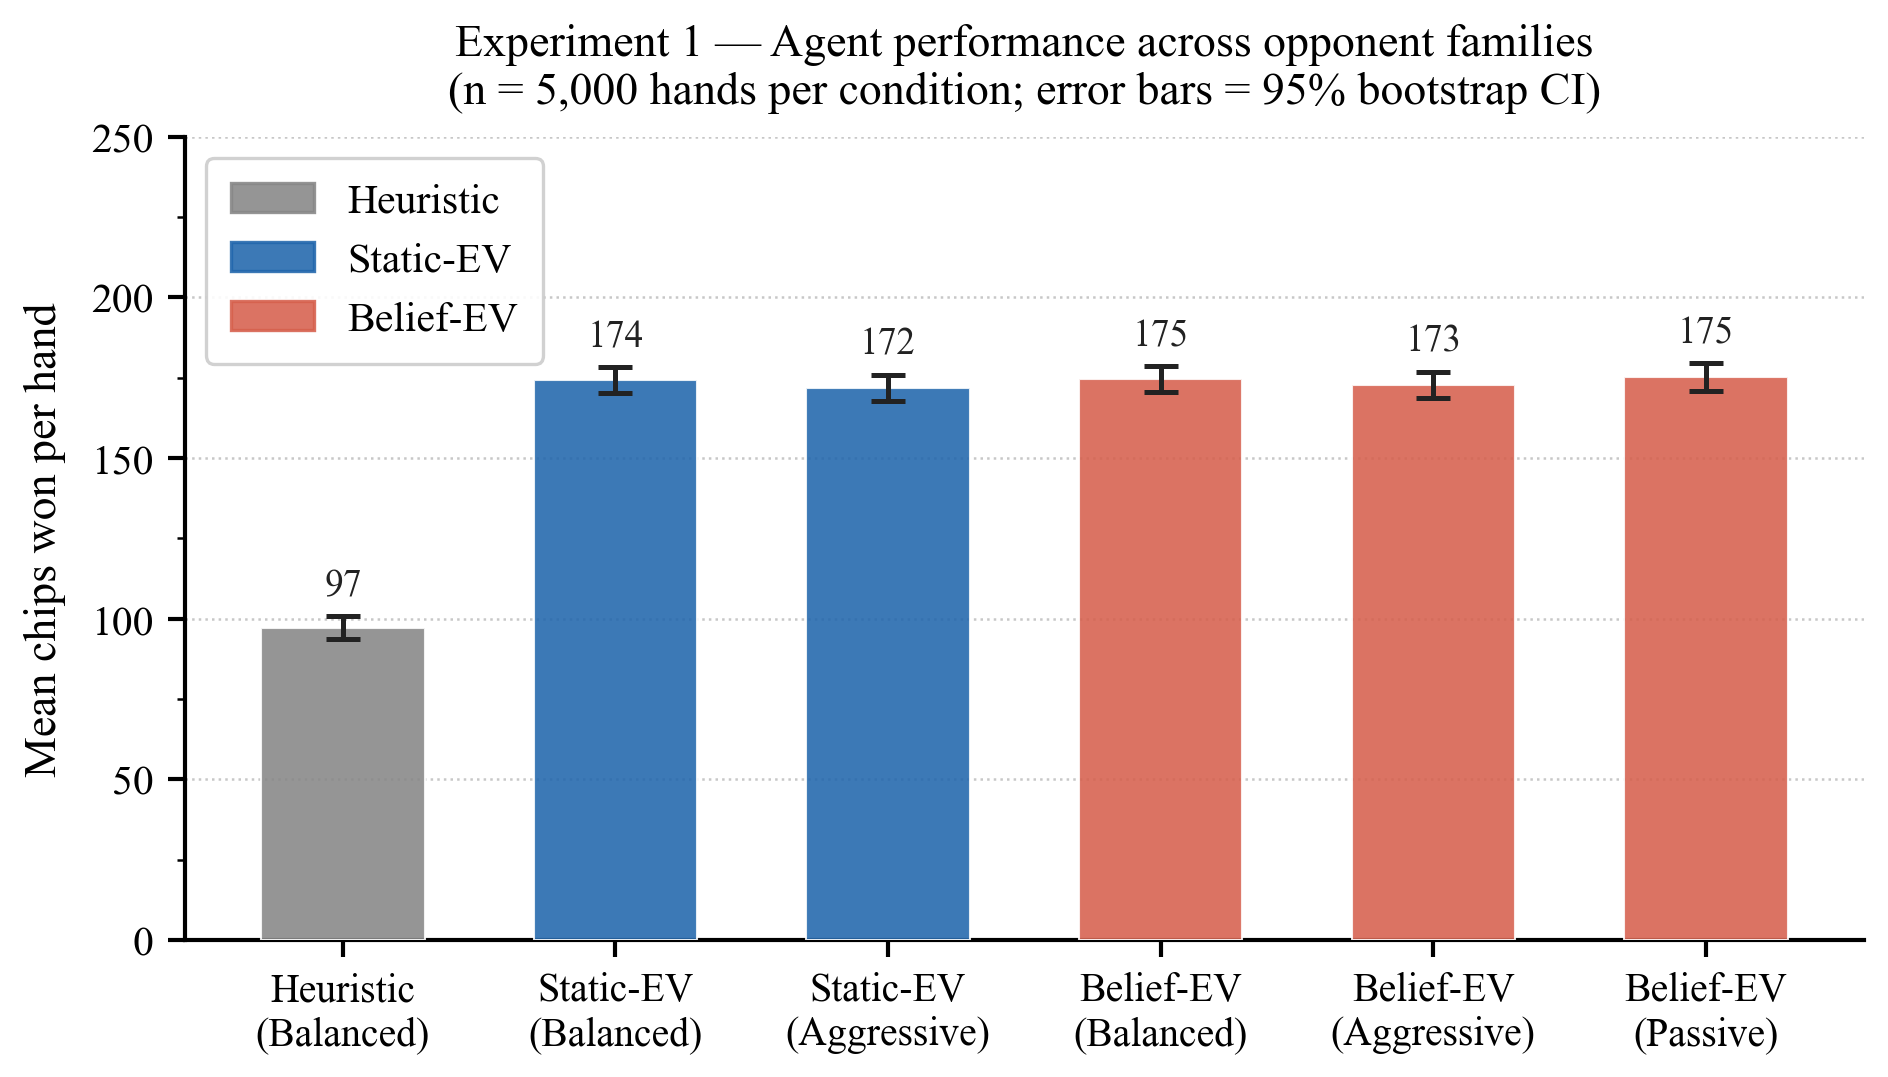
\includegraphics[width=0.92\textwidth]{figures/fig1_main_comparison.png}
  \caption{%
    \textbf{Experiment 1 -- Agent performance across opponent families.}
    Mean chips won per hand (player~0) for the Heuristic, Static-EV,
    and Belief-EV agents under six conditions.
    Error bars: 95\% bootstrap CI ($n=5{,}000$ per condition;
    five seeds $\times$ 1,000 hands).
    Both EV agents outperform the Heuristic by $\approx$77 chips/hand
    ($\approx$79\%); the Belief-EV vs.\ Static-EV gap is $\leq$1
    chip/hand in all conditions.
    Grey = Heuristic; blue = Static-EV; orange-red = Belief-EV.
  }
  \label{fig:main_comparison}
\end{figure}

\begin{table}[ht]
  \centering
  \small
  \caption{%
    \textbf{Experiment 1 -- Summary statistics for all conditions.}
    Mean $\pm$ SD chips/hand (player~0), 95\% bootstrap CI, and
    $n$.
    Both EV agents outperform the Heuristic consistently;
    Belief-EV and Static-EV are within 1 chip/hand of each other
    when both face a Heuristic opponent.
  }
  \label{tab:main_results}
  \begin{tabularx}{\textwidth}{l l l
    S[table-format=3.1]
    S[table-format=3.1]
    @{\,}c@{\,}
    S[table-format=3.1]
    S[table-format=5.0]}
    \toprule
    Agent & Opponent family & Matchup &
    {Mean} & {SD} & {95\% CI} & {} & {$n$} \\
    \midrule
    Heuristic  & Balanced   & vs.\ Heuristic & 97.2  & 123.7 & [93.8,  & 100.8] & 5000 \\
    Static-EV  & Balanced   & vs.\ Heuristic & 174.2 & 148.7 & [170.1, & 178.3] & 5000 \\
    Static-EV  & Aggressive & vs.\ Heuristic & 171.8 & 147.3 & [167.9, & 175.9] & 5000 \\
    Belief-EV  & Balanced   & vs.\ Heuristic & 174.6 & 147.8 & [170.4, & 178.7] & 5000 \\
    Belief-EV  & Aggressive & vs.\ Heuristic & 172.8 & 146.4 & [168.8, & 176.9] & 5000 \\
    Belief-EV  & Passive    & vs.\ Heuristic & 175.2 & 151.5 & [171.0, & 179.5] & 5000 \\
    \bottomrule
  \end{tabularx}
\end{table}

\FloatBarrier

\subsection{Experiment 2: Static-EV Outperforms Belief-EV in Direct Competition}

Figure~\ref{fig:belief_ablation} shows the distribution of per-hand
chip differentials (Belief-EV $-$ Static-EV) in head-to-head play.
Table~\ref{tab:ablation_results} reports means, confidence intervals,
and test statistics.

Static-EV wins significantly more chips/hand than Belief-EV in two
of three conditions:
$-13.1$ chips/hand on the trappy family
($t(4999)=-2.36$, $p=0.018$)
and $-11.9$ chips/hand on the aggressive family
($t(4999)=-2.12$, $p=0.034$).
The balanced-family difference of $-9.9$ chips/hand is in the same
direction but does not reach conventional significance
($t(4999)=-1.76$, $p=0.078$).
Effect sizes of $\approx$10--13 chips/hand represent approximately
6--7\% of the mean pot.

\textbf{This constitutes a falsification of the central hypothesis.}
Belief updating does not improve payoff in direct competition; it
imposes a measurable cost.
We attribute this to response-model misspecification: the Bayesian
update in Equation~\ref{eq:bayes_update} amplifies errors in
$P(a \mid c,\, s,\, \mathcal{F})$ when the opponent is itself
EV-rational rather than drawn from the assumed family.

\begin{figure}[ht]
  \centering
  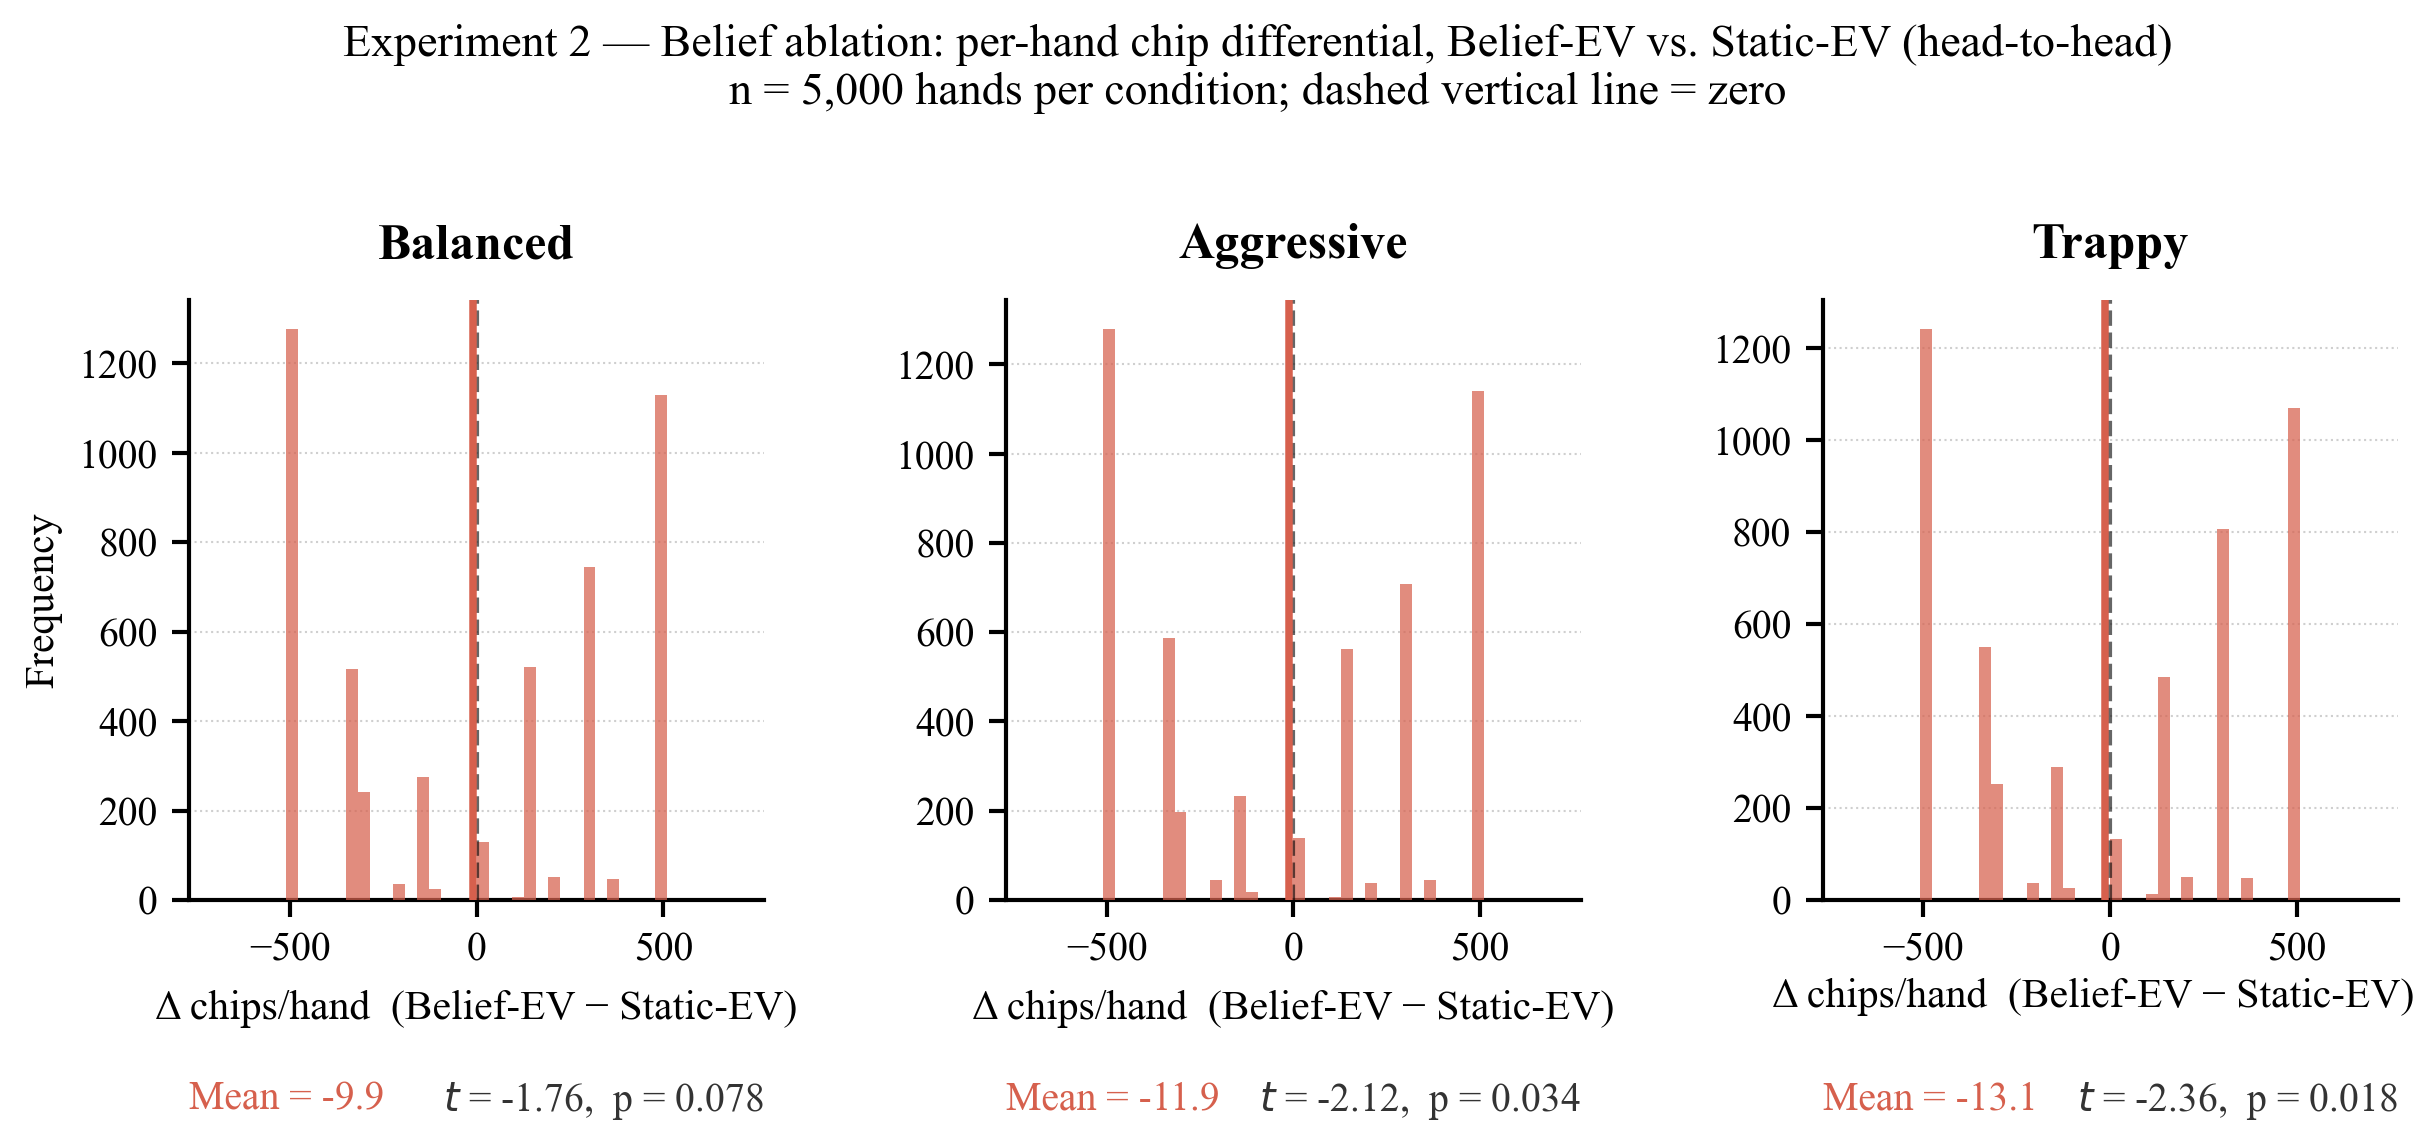
\includegraphics[width=0.98\textwidth]{figures/fig2_belief_ablation.png}
  \caption{%
    \textbf{Experiment 2 -- Belief ablation: per-hand chip differentials,
    Belief-EV vs.\ Static-EV (head-to-head).}
    Histograms of the per-hand chip difference
    (Belief-EV $-$ Static-EV) across 5,000 hands for the balanced,
    aggressive, and trappy opponent contexts.
    Solid coloured vertical line = empirical mean;
    dashed black line = zero.
    In all three conditions the mean is negative, indicating that
    Static-EV wins more chips/hand.
    Annotations below the $x$-axis report empirical mean and
    paired $t$-test statistics.
  }
  \label{fig:belief_ablation}
\end{figure}

\begin{table}[ht]
  \centering
  \small
  \caption{%
    \textbf{Experiment 2 -- Belief ablation results.}
    Mean chips/hand for Belief-EV (player~0) and Static-EV
    (player~1), mean difference with 95\% bootstrap CI, and
    paired $t$-test statistics.
    Negative differences favour Static-EV.
    $n=5{,}000$ per condition.
  }
  \label{tab:ablation_results}
  \begin{tabularx}{\textwidth}{l
    S[table-format=3.1]
    S[table-format=3.1]
    S[table-format=3.1]
    @{\,}c@{\,}
    S[table-format=3.1]
    S[table-format=-1.2]
    S[table-format=1.4]}
    \toprule
    Context &
    {Belief} & {Static} & {\multicolumn{3}{c}{Diff [95\% CI]}} &
    {$t$} & {$p$} \\
    \midrule
    Balanced    & 184.5 & 194.4 & -9.9  & [&$-20.5,\, +1.0$&] & -1.76 & 0.0778 \\
    Aggressive  & 184.3 & 196.1 & -11.9 & [&$-22.5,\, -0.8$&] & -2.12 & 0.0342 \\
    Trappy      & 181.3 & 194.4 & -13.1 & [&$-23.8,\, -2.2$&] & -2.36 & 0.0183 \\
    \bottomrule
  \end{tabularx}
\end{table}

\FloatBarrier

\subsection{Experiment 3: Posterior Entropy and Behavioural Profiles}

Figure~\ref{fig:calibration} (left) shows posterior entropy
distributions.
Mean entropy is nearly identical across families:
$H=1.914$ bits (balanced), $1.914$ bits (aggressive), $1.913$ bits
(maniac) -- all within $0.033$ bits of the maximum
$H_{\max}=\log_2 7 \approx 1.946$ bits.
Standard deviations are $\sigma \leq 0.07$ bits.
These near-maximal values indicate that observing a single opponent
action provides negligible information for discriminating among the
seven hand classes, consistent with theoretical expectations for
poorly identified latent-variable models\cite{gal2016dropout,
murphy2012ml}.

Figure~\ref{fig:calibration} (right) shows action frequency profiles.
The Heuristic checks on 55.1\% of decisions and jams on only 1.2\%.
Static-EV and Belief-EV are nearly indistinguishable: both bet
half-pot on $\approx$44--45\% of decisions and jam on
$\approx$28--29\%.
The near-identical profiles confirm that posterior updating is not
generating meaningfully different action selections.

\begin{figure}[ht]
  \centering
  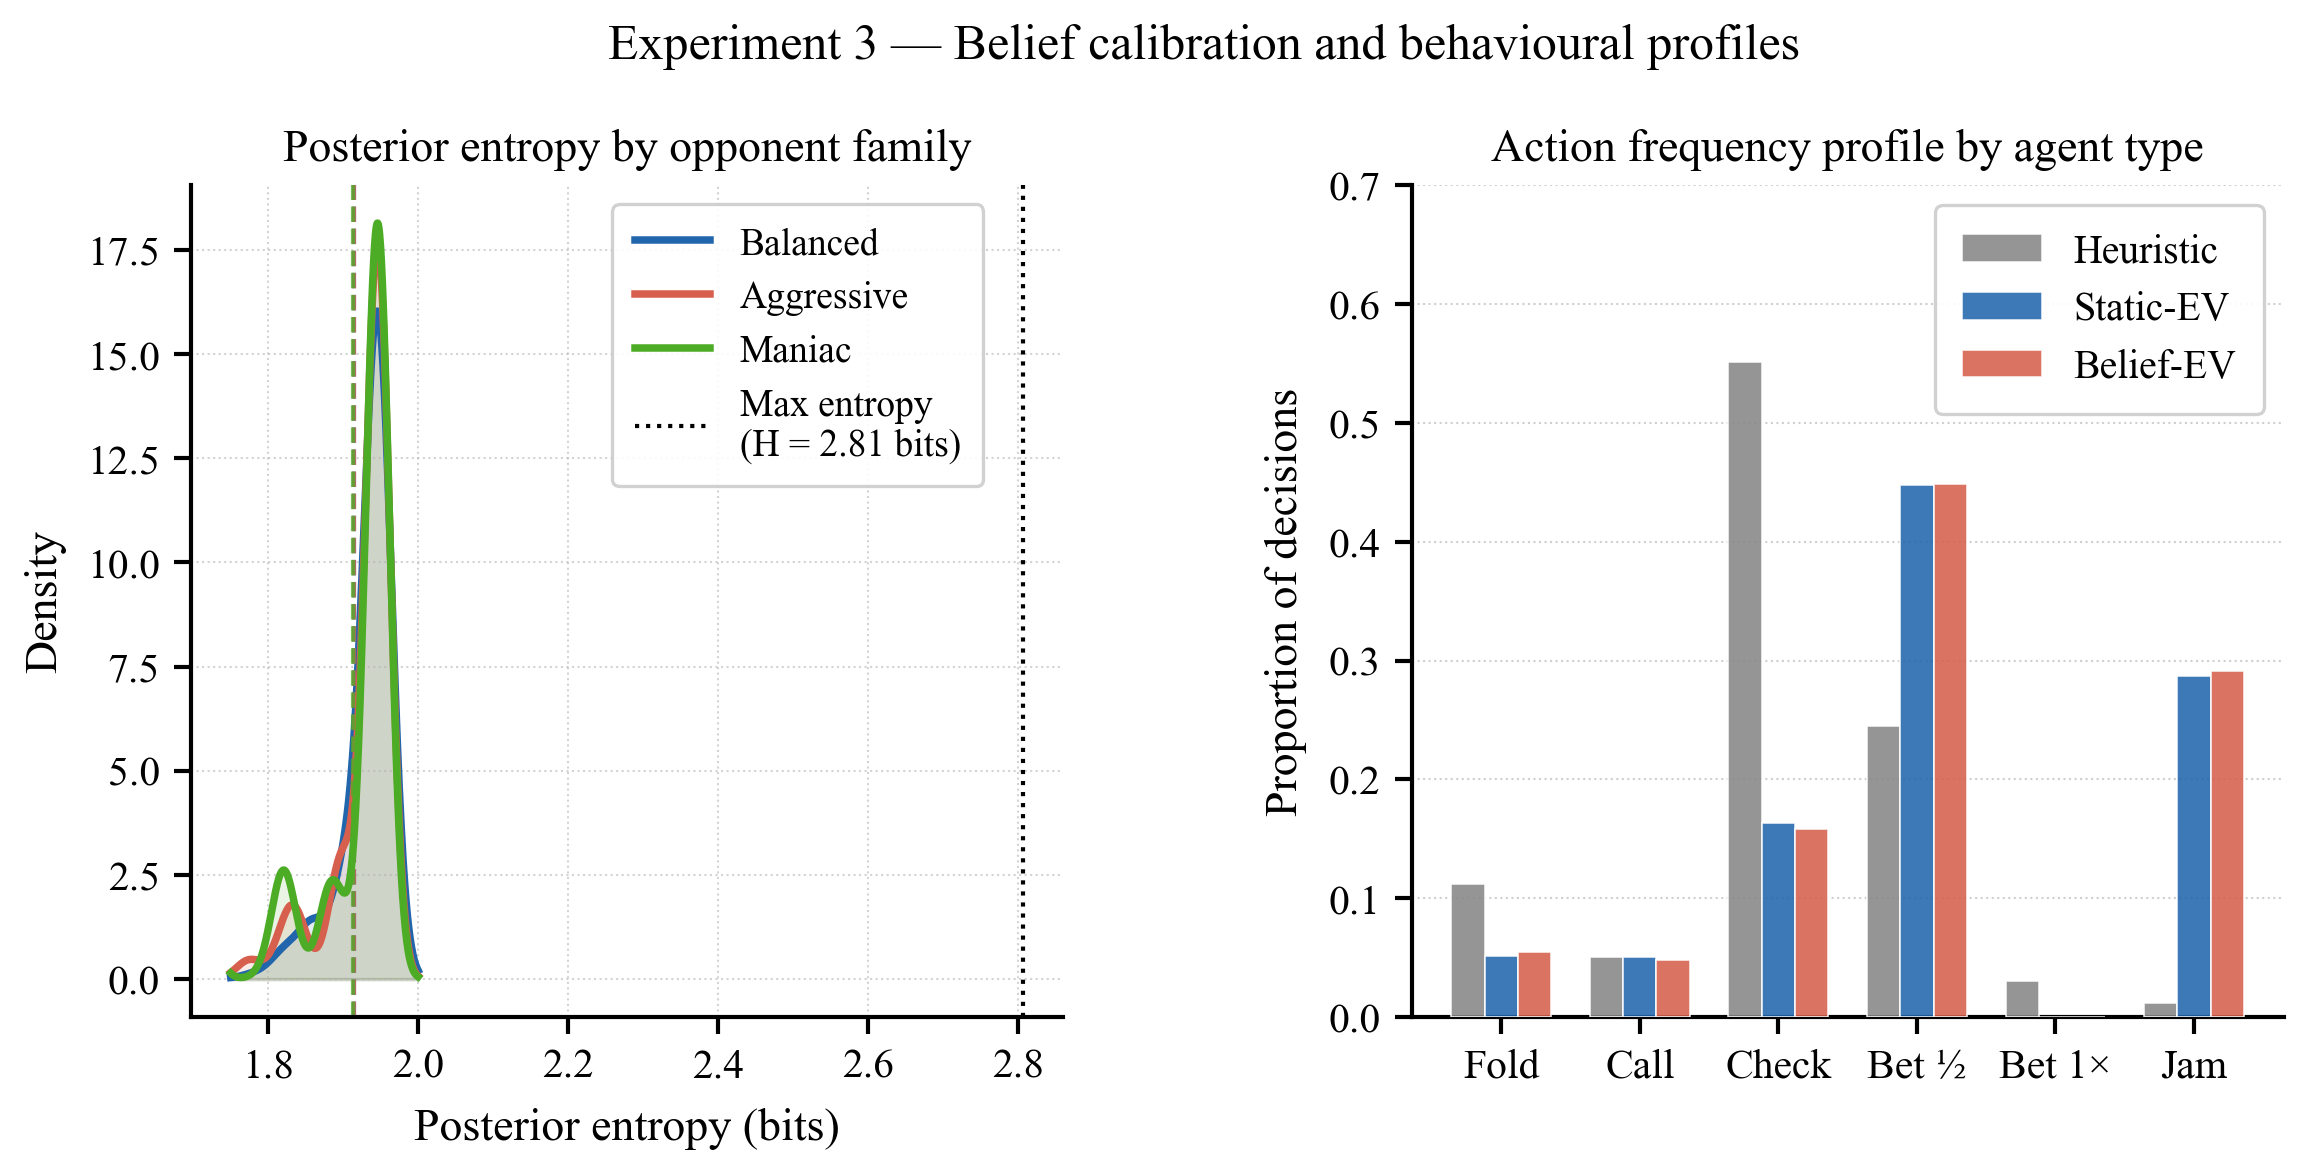
\includegraphics[width=0.96\textwidth]{figures/fig3_calibration.png}
  \caption{%
    \textbf{Experiment 3 -- Posterior entropy and action frequency profiles.}
    \textit{Left}: KDE of per-decision posterior entropy (bits) for the
    Belief-EV agent under balanced (blue), aggressive (orange), and
    maniac (green) opponent families.
    Dashed vertical lines = family means;
    dotted black line = maximum entropy
    ($H_{\max}=\log_2 7 \approx 1.946$ bits).
    All distributions cluster near $H_{\max}$, indicating the
    posterior remains close to uniform.
    \textit{Right}: Action frequency profiles for all three agents
    (balanced opponent; $n=5{,}000$ hands each).
    Static-EV and Belief-EV profiles are nearly identical;
    the Heuristic is substantially more passive.
  }
  \label{fig:calibration}
\end{figure}

\begin{table}[ht]
  \centering
  \small
  \caption{%
    \textbf{Experiment 3 -- Posterior entropy and action frequencies.}
    Mean $\pm$ SD posterior entropy (bits) per decision for the
    Belief-EV agent; action proportions for each agent type
    (balanced opponent; $n=5{,}000$ hands).
  }
  \label{tab:calibration}
  \begin{tabularx}{0.75\textwidth}{l l
      S[table-format=1.3]@{\,$\pm$\,}S[table-format=1.3]}
    \toprule
    \multicolumn{2}{l}{Posterior entropy} &
    \multicolumn{2}{c}{Mean $\pm$ SD (bits)} \\
    \midrule
    & Balanced   & 1.914 & 0.074 \\
    & Aggressive & 1.914 & 0.066 \\
    & Maniac     & 1.913 & 0.064 \\
    \bottomrule
  \end{tabularx}
  \vspace{6pt}
  \begin{tabularx}{0.75\textwidth}{l
      S[table-format=1.3] S[table-format=1.3] S[table-format=1.3]
      S[table-format=1.3] S[table-format=1.3]}
    \toprule
    Agent & {Fold} & {Call} & {Check} & {Bet$\tfrac{1}{2}$} & {Jam} \\
    \midrule
    Heuristic  & 0.112 & 0.050 & 0.551 & 0.245 & 0.012 \\
    Static-EV  & 0.052 & 0.050 & 0.163 & 0.447 & 0.287 \\
    Belief-EV  & 0.054 & 0.048 & 0.158 & 0.448 & 0.292 \\
    \bottomrule
  \end{tabularx}
\end{table}

\FloatBarrier

\subsection{Experiment 4: Robustness to Held-Out Opponent Families}

Figure~\ref{fig:robustness} compares development and held-out
performance for all three agents.
Neither EV agent shows a meaningful drop on held-out families.
Belief-EV: $+0.76$ chips/hand on held-out~1 and $+0.58$ on
held-out~2.
Static-EV: $-0.58$ on held-out~1 and $+2.21$ on held-out~2.
All $|\Delta| \leq 2.2$ chips/hand, negligible relative to the
$\approx$150-chip per-hand standard deviation.
\textbf{The Belief-EV agent gains no robustness advantage over
Static-EV} despite maintaining an explicit dynamic belief model,
consistent with the near-uniform posteriors in Experiment~3.

\begin{figure}[ht]
  \centering
  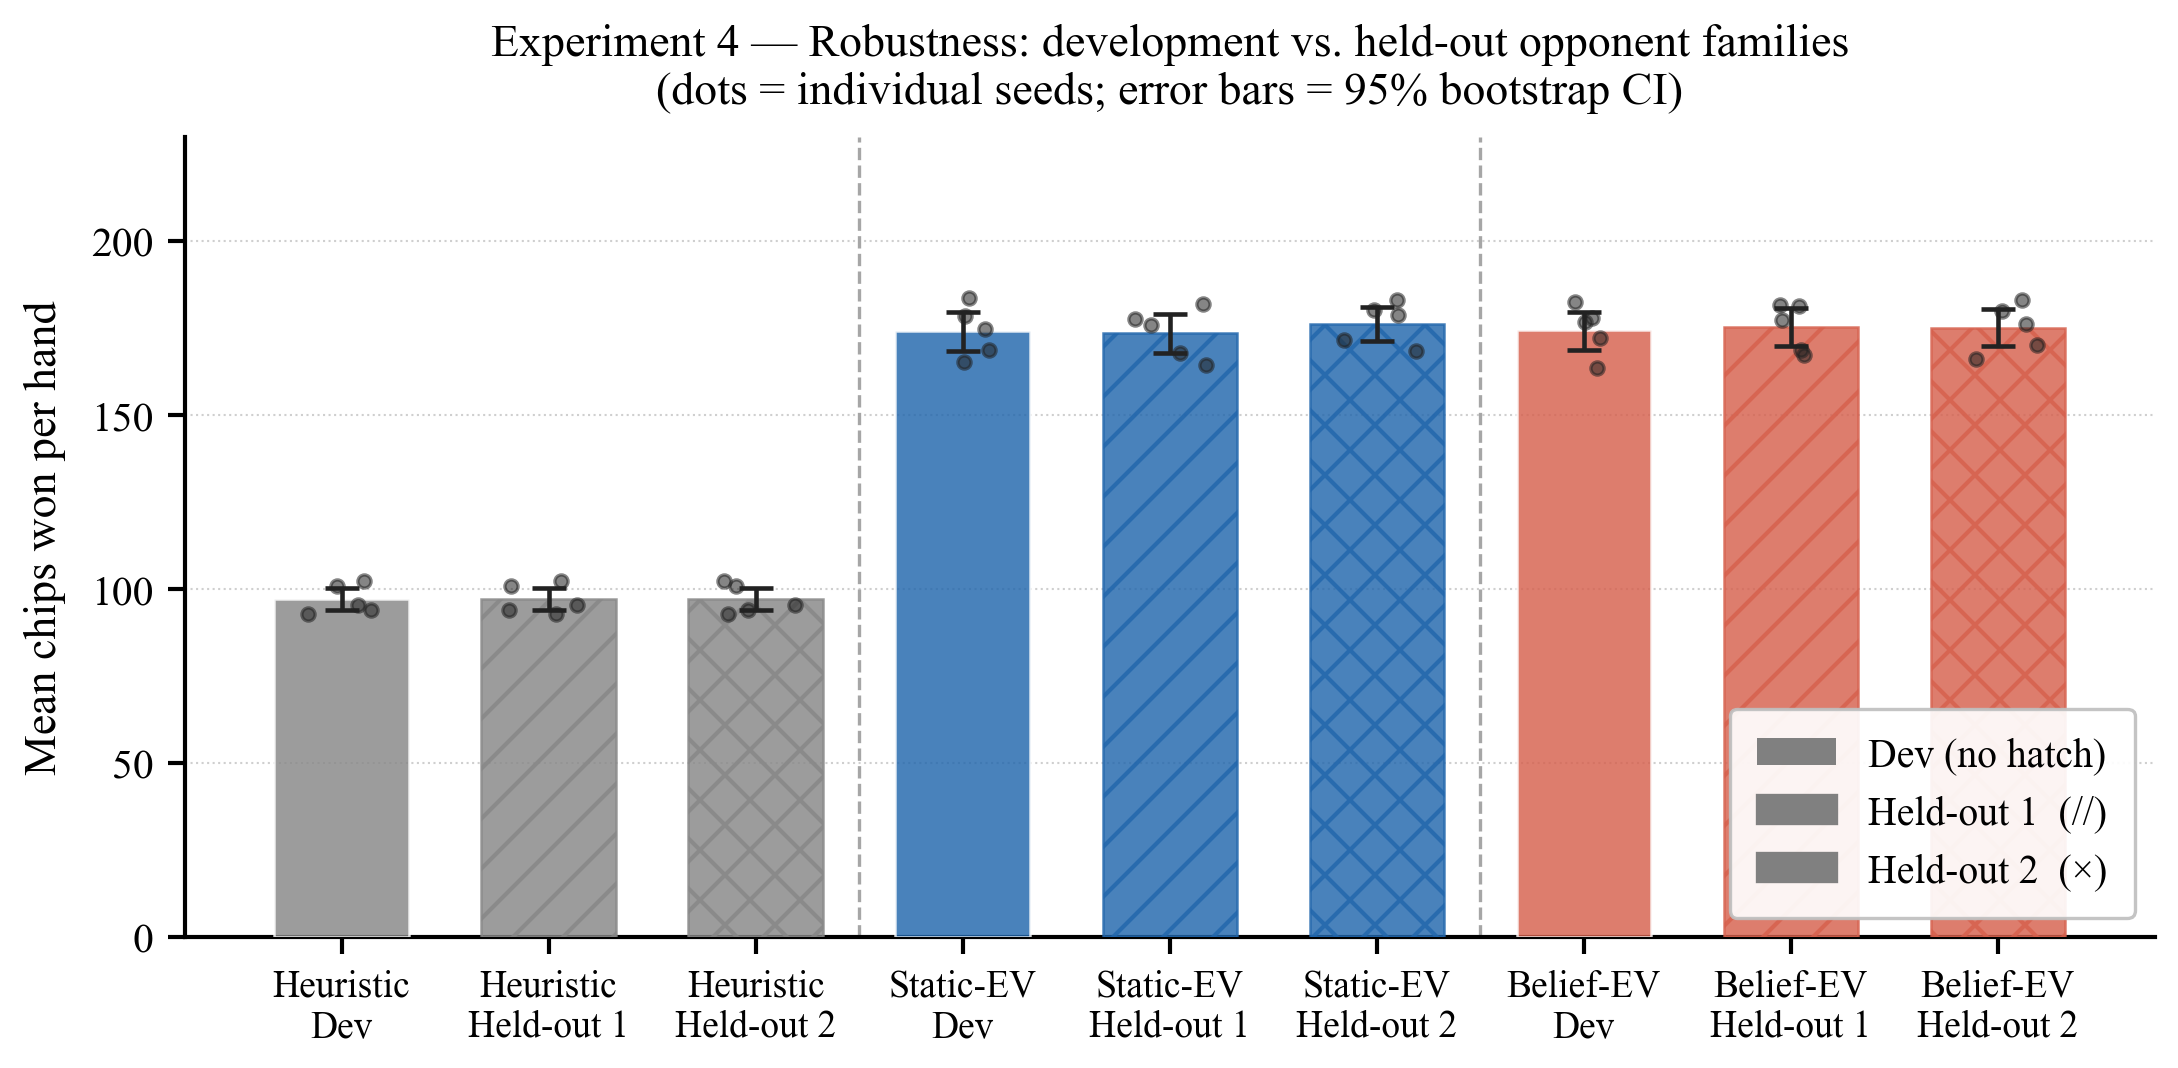
\includegraphics[width=0.96\textwidth]{figures/fig4_robustness.png}
  \caption{%
    \textbf{Experiment 4 -- Robustness to held-out opponent families.}
    Mean chips/hand for all three agents on development (no hatch),
    held-out~1 (forward-slash), and held-out~2 (cross-hatch) families.
    Dots = seed-level means; error bars = 95\% bootstrap CI.
    Neither EV agent shows a performance drop; Belief-EV provides
    no robustness advantage over Static-EV.
    Vertical dashed lines separate agent groups.
  }
  \label{fig:robustness}
\end{figure}

\begin{table}[ht]
  \centering
  \small
  \caption{%
    \textbf{Experiment 4 -- Robustness summary.}
    Mean chips/hand on development (Dev) and held-out families
    with 95\% bootstrap CI.
    $\Delta$ = change from development baseline.
    All $|\Delta| \leq 2.2$ chips/hand.
    $n=5{,}000$ per cell.
  }
  \label{tab:robustness_results}
  \begin{tabularx}{0.75\textwidth}{l l
      S[table-format=3.1]
      @{\,}c@{\,}
      S[table-format=3.1]
      S[table-format=+1.1]}
    \toprule
    Agent & Family &
    {Mean} & {95\% CI} & {} & {$\Delta$ Dev} \\
    \midrule
    Heuristic
      & Dev         & 97.2  & [93.8,  & 100.8] &       0.0 \\
      & Held-out 1  & 97.2  & [93.8,  & 100.8] &      +0.0 \\
      & Held-out 2  & 97.2  & [93.8,  & 100.8] &      +0.0 \\[3pt]
    Static-EV
      & Dev         & 174.2 & [170.1, & 178.3] &      ref. \\
      & Held-out 1  & 173.6 & [169.5, & 177.5] &      -0.6 \\
      & Held-out 2  & 176.4 & [172.2, & 180.5] &      +2.2 \\[3pt]
    Belief-EV
      & Dev         & 174.6 & [170.4, & 178.7] &      ref. \\
      & Held-out 1  & 175.4 & [171.3, & 179.5] &      +0.8 \\
      & Held-out 2  & 175.2 & [171.0, & 179.3] &      +0.6 \\
    \bottomrule
  \end{tabularx}
\end{table}

\FloatBarrier

\subsection{Seed-Level Stability}

Figure~\ref{fig:seed_variance} plots per-seed means across five
replications.
The Heuristic varies between 91 and 103 chips/hand; both EV agents
between 163 and 184 chips/hand.
Agent rank ordering is preserved in all five seeds and the
Belief-EV vs.\ Static-EV difference never reverses sign, confirming
the main findings are not seed artifacts.

\begin{figure}[ht]
  \centering
  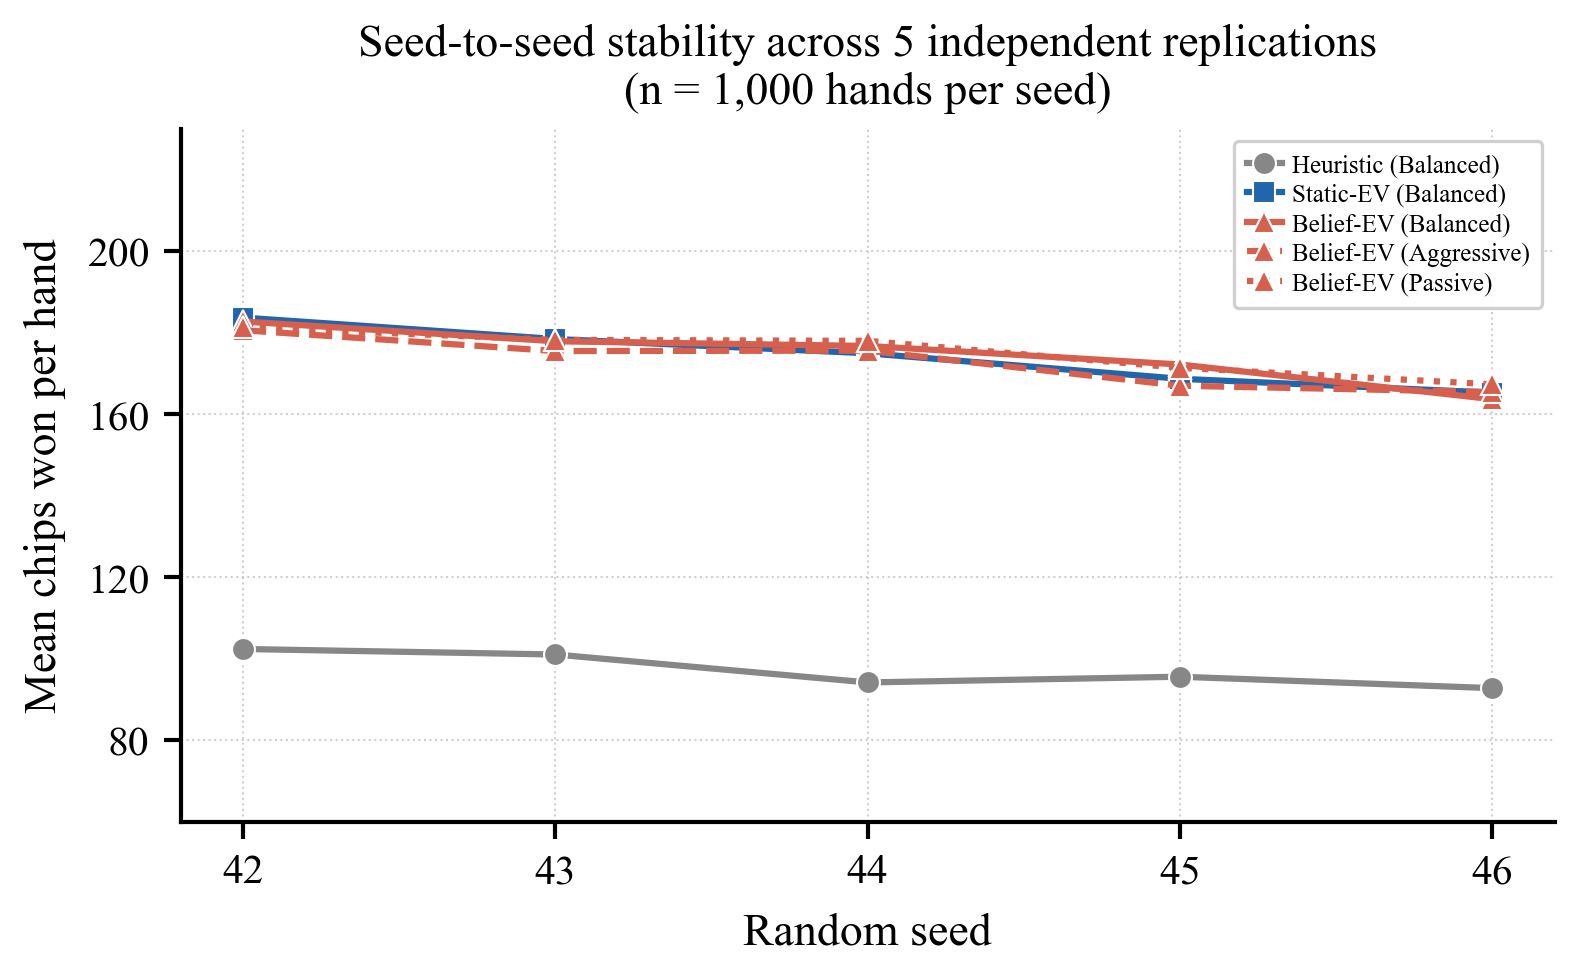
\includegraphics[width=0.75\textwidth]{figures/fig5_seed_variance.png}
  \caption{%
    \textbf{Seed-to-seed stability across five independent replications.}
    Mean chips/hand plotted against random seed.
    Circles = Heuristic; squares = Static-EV; triangles = Belief-EV.
    Line style encodes opponent family (solid = balanced,
    dashed = aggressive, dotted = passive).
    Agent rank ordering is preserved across all seeds.
    $n=1{,}000$ hands per seed.
  }
  \label{fig:seed_variance}
\end{figure}

\FloatBarrier

\subsection{Summary of Findings}

Table~\ref{tab:summary} synthesises the four experiments.

\begin{table}[ht]
  \centering
  \small
  \caption{%
    \textbf{Summary of all experimental findings.}
    $\uparrow$/$\downarrow$ = outperforms/underperforms reference;
    $\approx$ = negligible difference.
  }
  \label{tab:summary}
  \begin{tabularx}{0.75\textwidth}{l l l l}
    \toprule
    Exp. & Comparison & Effect & Magnitude \\
    \midrule
    1 & EV vs.\ Heuristic        & $\uparrow$       & $+77$ chips/hand \\
    1 & Belief-EV vs.\ Static-EV & $\approx$        & $+0.4$ chips/hand \\
    2 & Belief-EV vs.\ Static-EV & $\downarrow$     & $-10$ to $-13$ ch/h \\
      & (head-to-head)           & ($p\leq0.034$)   & \\
    3 & Posterior entropy        & Near max         & $H\approx1.91$ bits \\
    3 & Action profiles          & $\approx$        & $<$1\% difference \\
    4 & EV robustness            & $\approx$        & $|\Delta|\leq2.2$ ch/h \\
    4 & Belief-EV robustness     & No advantage     & vs.\ Static-EV \\
    \bottomrule
  \end{tabularx}
\end{table}

%% ─────────────────────────────────────────────────────────────────────────────
%%  DISCUSSION
%% ─────────────────────────────────────────────────────────────────────────────
\section{Discussion}

\subsection{The Primacy of EV Reasoning}

The dominant empirical finding -- a $\approx$79\% chip-per-hand
advantage of EV agents over the Heuristic -- replicates a pattern
well known from the poker AI literature: structured expected-value
reasoning, even with a uniform prior, far outperforms fixed-rule
systems\cite{bowling2015holdem,brown2019superhuman}.
The result is robust to opponent family, random seed, and street
context, establishing principled EV computation as the critical
ingredient for decision quality in this setting.

This has a direct practical corollary.
In any domain where agents currently operate via hand-coded rules
or score-based thresholds -- clinical triage\cite{obermeyer2016predicting},
fraud scoring\cite{dalpozzolo2015fraud}, market-making spread
policies\cite{glosten1985bid} -- the transition to even a static
EV-aware framework is likely to yield the largest achievable gain.
Dynamic belief tracking is a second-order consideration.

\subsection{Why Belief Updating Fails Here}

The failure of the Belief-EV agent is mechanistically transparent.
Posterior entropy in Experiment~3 averages $H\approx1.91$ bits
against a maximum of $1.946$ bits -- the posterior is nearly
uniform at every decision point.
Three factors jointly explain this:

\begin{enumerate}[leftmargin=*, itemsep=1pt, topsep=2pt]
  \item \textbf{Low action discriminability.}
    Under the parameterised response model, different hand classes
    produce similar action probabilities, so the likelihood ratio
    $P(a \mid c_i)/P(a \mid c_j)$ is small and the update in
    Equation~\ref{eq:bayes_update} is weak.
  \item \textbf{Few observed actions.}
    A turn-river subgame generates at most two to four
    opponent actions per hand, providing too little data to
    substantially shift a seven-class posterior\cite{murphy2012ml}.
  \item \textbf{Opponent mismatch.}
    In Experiment~2, the Static-EV opponent does not follow the
    response model at all, so the Bayesian update is driven by
    a systematically wrong likelihood -- a canonical instance of
    model misspecification\cite{gal2016dropout}.
\end{enumerate}

The result is that the Belief-EV agent pays a constant computational
and implicit inference overhead (smoothing, per-class response
queries, EV reweighting) without receiving corresponding
discriminating signal.
When the noise in the posterior update exceeds the signal, the
update degrades rather than improves the action selection.
This is consistent with theoretical results on the value of
information under model
misspecification\cite{gal2016dropout,albrecht2018survey}.

\subsection{Robustness Without Belief}

The finding that both EV agents transfer equally to held-out
opponent families -- with neither agent showing robustness advantage
from dynamic belief tracking -- has a clean interpretation.
When the posterior is near-uniform, the Belief-EV and Static-EV
agents are functionally equivalent: both select actions based
approximately on a uniform prior over hand classes, and the
identity of the opponent family is therefore irrelevant to the
action taken.
Robustness in this regime is a property of the EV framework
itself, not of the belief-updating layer.

This contrasts with theoretical settings in which opponent
modelling is expected to improve generalisation, such as when
the response model is highly accurate and opponent families are
well-separated in behaviour space\cite{albrecht2018survey,
tuyls2012multiagent}.
Our results bound the conditions under which those gains
materialise: at minimum, the response model must assign
meaningfully different action probabilities to different latent
classes, and sufficient opponent actions must be observed.

\subsection{Implications for Applied Systems}

These findings speak directly to design choices in several
applied domains.

\textbf{AI agents and LLMs.}
An agent that maintains a dynamic model of user intent and updates
it after each message incurs inference overhead and misspecification
risk.
Our results suggest that a well-calibrated static prior plus
principled expected-value reasoning will match or exceed the
performance of a belief-updating layer in most practical
settings\cite{silver2016alphago,mnih2015dqn}.

\textbf{Fraud detection.}
Sequential transaction models that update account-state beliefs
offer marginal improvement over static risk scoring unless the
behavioural model of fraudster actions is highly accurate.
The heuristic-to-EV transition remains the dominant
gain\cite{dalpozzolo2015fraud}.

\textbf{Financial market making.}
The adverse-selection literature\cite{glosten1985bid} predicts
that market makers who accurately model informed-trader behaviour
will set tighter spreads.
Our results suggest that under response-model misspecification --
plausible when counterparties adapt strategically -- static
inventory-EV models may outperform dynamic belief-updating
overlays, consistent with practitioner preferences for simpler
models.

\textbf{Clinical decision support.}
Sequential Bayesian diagnostic models offer theoretical advantages
over static scoring systems\cite{obermeyer2016predicting},
but our results suggest the practical benefit depends critically
on whether the conditional disease-progression model is well
specified.
When it is not, static EV-calibrated scores may be safer and
more reliable.

\textbf{Autonomous vehicles.}
Intent-prediction modules that maintain dynamic beliefs about
driver behaviour are common in AV stacks\cite{bard2020hanabi}.
Our results indicate that static worst-case EV planning may
provide equivalent robustness if the intent model is weakly
discriminative -- a realistic condition in mixed urban traffic.

\subsection{Limitations}

Several limitations bound the generality of our conclusions.

First, the study uses a fully synthetic response model.
The finding that belief updating fails is partly a consequence of
the specific response-model parameters chosen; with a more
discriminative likelihood function, belief updates might yield
gains.
We regard this as a strength for internal validity but a limitation
for external generalisability.

Second, the action space is intentionally coarse.
A finer-grained bet-sizing tree would create more action diversity
and potentially more informative observations for belief updating.
Future work should test whether richer action abstractions
rehabilitate the Belief-EV agent.

Third, we test a single-level belief hierarchy.
Recursive reasoning -- modelling the opponent's model of us,
as in $k$-level thinking\cite{osborne1994course} -- is absent
from all three agents.
Higher-order belief structures may interact differently with
misspecification.

Fourth, the turn-river subgame excludes preflop and flop
decisions where range compression creates more informative
action signals.
The posterior may be more useful in richer game trees.

\subsection{Future Directions}

Several extensions follow naturally.
Varying response-model discriminability through sensitivity
analysis would map the boundary conditions under which belief
updating becomes beneficial.
Replacing the fixed parameterised response model with a learned
model (e.g., from observed hand histories) would test whether
data-driven likelihoods close the gap between Belief-EV and
Static-EV.
Finally, applying counterfactual regret minimisation\cite{zinkevich2007cfr}
as a fourth agent would contextualise both EV agents against
a game-theoretically optimal baseline.

%% ─────────────────────────────────────────────────────────────────────────────
%%  CONCLUSION
%% ─────────────────────────────────────────────────────────────────────────────
\section{Conclusion}

We have shown, in a controlled synthetic testbed, that principled
expected-value reasoning with a static prior produces dramatically
better decisions than rule-based heuristics ($+$77 chips/hand,
$\approx$79\%), but that adding Bayesian posterior updating over
opponent hand classes yields no additional gain and in fact imposes
a measurable performance cost of 10--13 chips/hand in direct
head-to-head competition ($p \leq 0.034$).
The mechanism is clear: when the response model cannot
discriminate among latent states, posterior entropy remains close
to its maximum and updates carry more noise than signal.
These findings falsify the common intuition that richer hidden-state
inference always improves decisions, and provide practitioners in
AI agent design, fraud detection, market making, and clinical
decision support with a concrete benchmark for evaluating the
expected benefit of dynamic belief-tracking systems before deploying
their additional complexity.

%% ─────────────────────────────────────────────────────────────────────────────
%%  REFERENCES
%% ─────────────────────────────────────────────────────────────────────────────
\newpage
\singlespacing
\bibliographystyle{unsrtnat}
\begin{thebibliography}{99}

\bibitem{osborne1994course}
Osborne, M.~J. \& Rubinstein, A.
\textit{A Course in Game Theory}.
MIT Press (1994).

\bibitem{pearl1988probabilistic}
Pearl, J.
\textit{Probabilistic Reasoning in Intelligent Systems}.
Morgan Kaufmann (1988).

\bibitem{chen2006mathematics}
Chen, B. \& Ankenman, J.
\textit{The Mathematics of Poker}.
ConJelCo LLC (2006).

\bibitem{bowling2015holdem}
Bowling, M., Burch, N., Johanson, M. \& Tammelin, O.
Heads-up limit hold'em poker is solved.
\textit{Science} \textbf{347}, 145--149 (2015).

\bibitem{brown2019superhuman}
Brown, N. \& Sandholm, T.
Superhuman AI for multiplayer poker.
\textit{Science} \textbf{365}, 885--890 (2019).

\bibitem{koller1992complexity}
Koller, D. \& Megiddo, N.
The complexity of two-person zero-sum games in extensive form.
\textit{Games Econ.\ Behav.} \textbf{4}, 528--552 (1992).

\bibitem{zinkevich2007cfr}
Zinkevich, M., Johanson, M., Bowling, M. \& Piccione, C.
Regret minimization in games with incomplete information.
\textit{Adv.\ Neural Inf.\ Process.\ Syst.} \textbf{20} (2007).

\bibitem{albrecht2018survey}
Albrecht, S.~V. \& Stone, P.
Autonomous agents modelling other agents: A comprehensive survey
and open problems.
\textit{Artif.\ Intell.} \textbf{258}, 66--95 (2018).

\bibitem{browne2012mcts}
Browne, C.~B. et al.
A survey of Monte Carlo tree search methods.
\textit{IEEE Trans.\ Comput.\ Intell.\ AI Games} \textbf{4},
1--43 (2012).

\bibitem{bard2020hanabi}
Bard, N. et al.
The Hanabi challenge: A new frontier for AI research.
\textit{Artif.\ Intell.} \textbf{280}, 103216 (2020).

\bibitem{silver2016alphago}
Silver, D. et al.
Mastering the game of Go with deep neural networks and tree search.
\textit{Nature} \textbf{529}, 484--489 (2016).

\bibitem{murphy2012ml}
Murphy, K.~P.
\textit{Machine Learning: A Probabilistic Perspective}.
MIT Press (2012).

\bibitem{gal2016dropout}
Gal, Y. \& Ghahramani, Z.
Dropout as a Bayesian approximation: Representing model uncertainty
in deep learning.
\textit{Proc.\ 33rd Int.\ Conf.\ Mach.\ Learn.} 1050--1059 (2016).

\bibitem{obermeyer2016predicting}
Obermeyer, Z. \& Emanuel, E.~J.
Predicting the future -- big data, machine learning, and clinical
medicine.
\textit{N.\ Engl.\ J.\ Med.} \textbf{375}, 1216--1219 (2016).

\bibitem{glosten1985bid}
Glosten, L.~R. \& Milgrom, P.~R.
Bid, ask and transaction prices in a specialist market with
heterogeneously informed traders.
\textit{J.\ Financ.\ Econ.} \textbf{14}, 71--100 (1985).

\bibitem{dalpozzolo2015fraud}
Dal~Pozzolo, A., Caelen, O., Johnson, R.~A. \& Bontempi, G.
Calibrating probability with undersampling for unbalanced
classification.
\textit{2015 IEEE Symp.\ Comput.\ Intell.\ Financ.\ Eng.\ Econ.}
1--7 (2015).

\bibitem{tuyls2012multiagent}
Tuyls, K. \& Weiss, G.
Multiagent learning: Basics, challenges, and prospects.
\textit{AI Mag.} \textbf{33}, 41--52 (2012).

\bibitem{mnih2015dqn}
Mnih, V. et al.
Human-level control through deep reinforcement learning.
\textit{Nature} \textbf{518}, 529--533 (2015).

\end{thebibliography}

\end{document}
